\section{Literature Review}\label{LitRev}

With the emergence of mobile device and mobile computing power, technologies offer us previously unimaginable global access to data, their theft prone property concurrently threatens our sense of control over data ownership. To protect the data stored on a mobile device in the case of loss or theft, today's users rely on traditional encrypted file systems, such as BitLocker and TrueCrypt \cite{MattB1993}. However, traditional encrypted file systems are often insufficient to protect mobile data for two reasons. First, such systems can and do fail in the real world for many reasons: users configure weak passwords or write their passwords on easily accessible sticky notes, decryption keys can be recovered from memory, and most of today's tamper resistant hardware can still be physically compromised \cite{JAlex2008}. Second, when traditional encryption fails, it fails silently. After a device is stolen, users have no way of knowing whether a thief has compromised their protections and accessed any sensitive files.

Such difficulties have led to the development of auditing file systems such as Keypad \cite{Roxana2011}, which supports fine-grained file access auditing that allows users to obtain explicit evidence of whether any files have been accessed after a device's loss as well as the ability to disable future file accesses after realizing that a device is lost. Keypad achieves these properties by weaving together encryption and remote encryption key management. Now Android smartphones amassed a commanding 68.1 market share of all mobile devices shipped during the second quarter of 2012 and operates under the Apache 2.0 open source license, which makes it an ideal candidate for a test bed of extension of Keypad design \cite{mobile2012}.

The following subsections introduce a number of key Android Operating System and Encryption key management concepts which were studied during the literature review. The current state of the field is then described, putting in context the possible contributions of this project. Finally, the research question driving this thesis is stated and a number of paths are presented for moving research forward.

\subsection{Key Concepts}\label{LitRevConcepts}

Prior to making any significant contributions to the field of auditing file system in mobile operating system security, a number of important and relevant concepts must first be examined and understood. The order of these concepts follows closely with the steps outlined for this project in Section \ref{Intro}. The technique that is used in Android to provide access for Android specific data is first considered. The design used by Keypad for remote key management that will be incorporated in this design is then explained. Finally, the ideas behind the encryption technique for database entries are outlined.

\subsubsection{Content Provider Class and Implementation}\label{LitRevConPro}

Android specific data are personal information of the users handled by system applications. These  system applications include: PackageManager, Calender, Contacts, Downloads, Bookmarks, CallLogs, Gmail, SMS, and User Dictionary. User data are managed and stored as database entries in SQLite database stored locally on the mobile device.

SQLite is an opensource, serverless, self-contained database implementation in C \cite{sqlite2000}. Android implemented SQLite in the Native layer as part of its library, and on top of that, a Java wrapper layer in its application framework. Android provided serval ways for an application to interact with this database as outlined in Table \ref{table:LitRevTableDbInteract}.

\begin{table}[ht]
\caption{Methods for Android Application to Interact with SQLite Database}
\centering
\begin{tabular}{l p{13cm}}
\hline\hline
Method & Description \\
\hline \\
SQLiteHelper & Create \textit{SQLiteDatabase} -$>$ Create an 
\textit{ApplicationDatabaseHelper} which extends \textit{SQLiteOpenHelper} -$>$ Call super class constructor with database name -$>$ Interact with the database with \textit{SQLiteDatabase.execSQL()}  \\ [1ex]
ContentProvider & Designing Content URIs -$>$ Implementing the \texti{ContentProvider} Class -$>$ Query the \textit{ContentProvider} through \textit{ContentResolver} Class  \\ [1ex]
\hline
\end{tabular}
\label{table:LitRevTableDbInteract}
\end{table}

If the database is completely local, application will employ \textit{SQLiteHelper} method. This class does the heavy lifting of creating and interacting with the database for the application, while the application can execute arbitrary queries through the \textit{SQLiteDatabase.execSQL()} method.

Applications that needs to store complex database schema and would also like to share its database content with other applications, interact with the SQLite database through an application framework \textit{ContentProvider}. It is a primary building block of Android application, and have been part of the Android system since API level 1. 

ContentProvider provides a series of abstract methods to be implemented by developers to allow flexibility and customization for each application: query(); insert(); update(); delete(); getType(); onCreate().

To better understand this concept, Figure \ref{FigContentProvider} demonstrates the hierarchical relationship between application and its provider class. In the Contact application, ContactProvider implements ContentProvider class to provide specific ways the Contact application wants to interact with the database that stores contact information. Contact application interacts with ContentProvider through ContentResolver, which takes an Uri object that maps query request to objects in the database.

\begin{figure}[h]
  \centering
  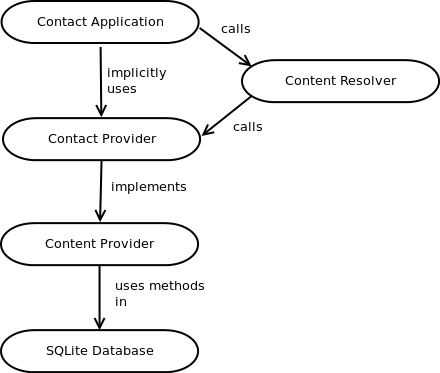
\includegraphics[scale=0.65]{./Figs/contact_provider.png}
  \caption
  {Provider hierarchy for Contact Application}
  \label{FigContentProvider}
\end{figure}

\subsubsection{Auditing File System for Android Specific Data}\label{LitRevAudit}

Auditing File System is a method of storing encryption key on a remote server for local data that is encrypted \cite{Cohen1997}. The advantage of this method is that each time a local file is accessed, the encryption key is fetched from the remote server, thus can be logged. Also, if the local data storage is compromised, key access can be disabled remotely thus preventing all future access.

\begin{figure}[h]
  \left
  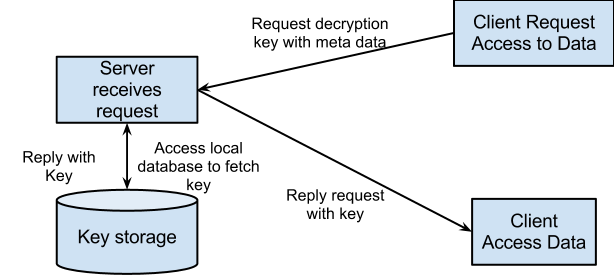
\includegraphics[scale=0.65]{./Figs/remote_key_storage.png}
  \caption
  {Request map for Remote Encryption Key Storage and Management}
  \label{FigRemoteKeyStorage}
\end{figure}

At time of data creation, the data is encrypted, and the key is sent to a remote audit service. As out lined in Figure \ref{FigRemoteKeyStorage}, when client request access to a piece of data, the key is then fetched from the server. Each piece of local data is encrypted with its own symmetric key. Client downloads the key for a file each time it is accessed, and destroys the key immediately after use.

To properly implement this method, several area needs to be well thought out. First of all, to manage the key stored on remote side efficiently, a database schema specific for the application for key storage needs to be implemented. Second of all, the request should contain minimal information such that the network usage is minimized. Third of all, server should be able to handle concurrent requests for concurrent data access. These aspects will be properly addressed in Section \ref{Progress}.

\subsubsection{Per-row vs Per-column encryption}\label{LitRevEnc}

To encrypt entries of database, and remotely manage its keys, we need to explore the benefit of different encryption schemes. As will be shown, per-row encryption allows fine-grain auditability but requires complete duplication of unencrypted database on the server side, while per-column encryption allow coarse-grain auditability, but only requires duplication of database schema on the server side. For each method, we will look at how database query will be implemented on a sample contact application.

\paragraph{Per-row encryption}\label{LitRevEncRow}

This method encrypts each row with a unique encryption key. The client side database will have each row encrypted with an unique encryption ID. Since querying an encrypted database directly is impossible, a copy of the unencrypted database is maintained on the server side with encryption id as well as decryption key. The sample database schema is outlined below.

Server: (EncID, Name, Email, Age, Key)

Client: (EncID, Name, Email, Age)

As shown in Figure \ref{FigRowInsert} Insert will be performed twice, once with unencrypted data on the server side, and second time with encrypted data on the device side.

\begin{figure}[h]
  \centering
  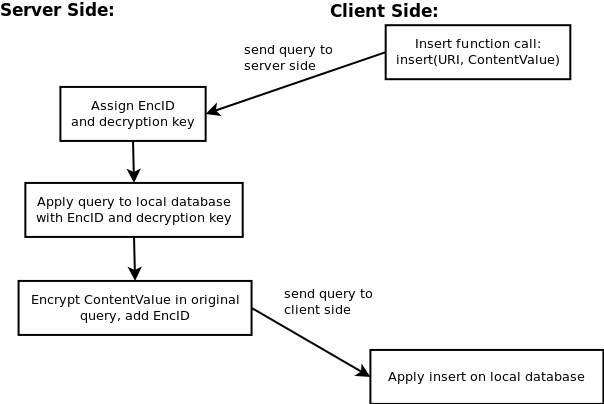
\includegraphics[scale=0.45]{./Figs/row_insert.png}
  \caption
  {Requset map of Insert method call for Per-Row encryption method}
  \label{FigRowInsert}
\end{figure}

As shown in Figure \ref{FigRowQuery}, two different type of query will be implemented with different logic. When the query involves a simple projection, a similar project on the column of decryption key is replied. Projection with selection requires us to find the specific EncID first, then send it back to the client side for the data to be queried and decrypted.

\begin{figure}[h]
  \centering
  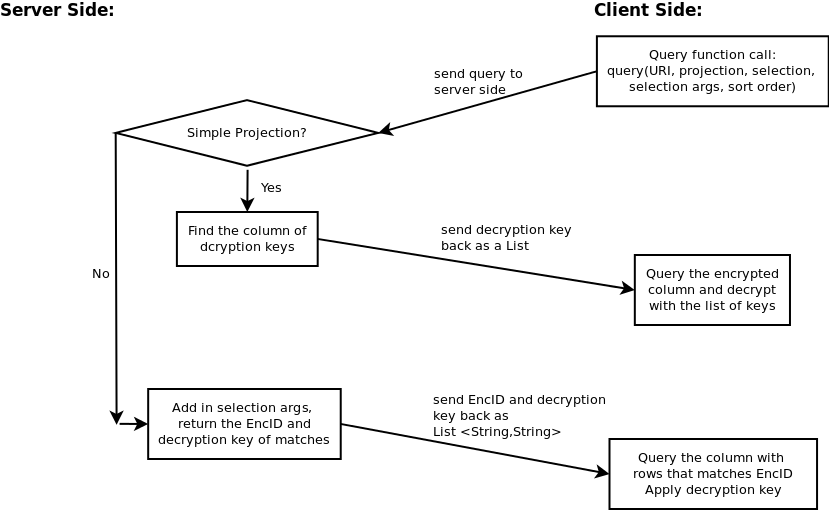
\includegraphics[scale=0.45]{./Figs/row_query.png}
  \caption
  {Requset map of Query method call for Per-Row encryption method}
  \label{FigRowQuery}
\end{figure}

\paragraph{Per-column encryption}\label{LitRevEncCol}

This method encrypts each column with an unique encryption key. The client side database will have each column encrypted. The server side database will simply maintain a list of decryption key for each column.

Server: (Column, Name, Key)

Client: (Name, Email, Age)

Since every column uses the same encryption key we simply need to request the key maintained on the server side and encrypt the data entries inserted into local database as outline in Figure \ref{FigColInsert}.

\begin{figure}[h]
  \centering
  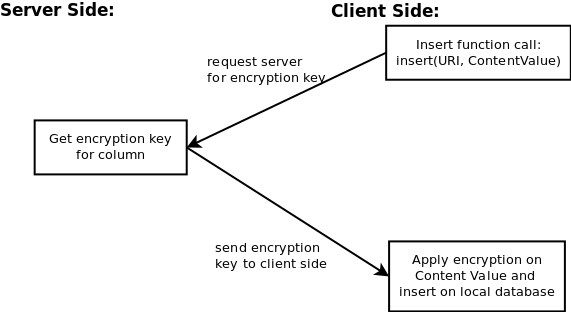
\includegraphics[scale=0.45]{./Figs/col_insert.png}
  \caption
  {Requset map of Insert method call for Per-Column encryption method}
  \label{FigColInsert}
\end{figure}

Since there is no way for us to query on encrypted data, we will decrypt the entire column, and perform query as outline in Figure \ref{FigColQuery}. After the query is completed we re-encrypt the entire column. This is similar to having an decryption key expired on a documented that is encrypted.

\begin{figure}[h]
  \centering
  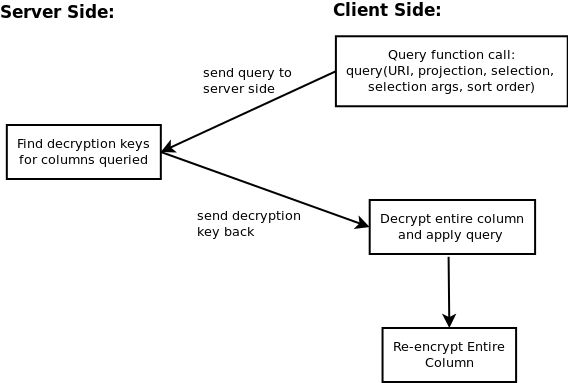
\includegraphics[scale=0.45]{./Figs/col_query.png}
  \caption
  {Requset map of Query method call for Per-Column encryption method}
  \label{FigColQuery}
\end{figure}

\subsection{Current State of Field}\label{LitRevCurrent}

To properly understand the current state of field relavent to this research, we first realize that the method employed is a combination of database encryption and remote key management.

Database encryption is a well explored topic. \textit{CryptDB} for example, is an open source database management system (DBMS) that operates on an encrypted database. It associates user password with the queries they performed directly on encrypted data. As a result, user can only view data relavent to themselves \cite{popa2011}. This solves the problem when a database administrator may want to access private data such as health record, as well as the situation when the entire DBMS is compromised. It works by realizing the idea that all SQL queries are made up of a set of well defined operators such as equals, orders and joins. It uses known encryption schems and privacy-preserving cryptographic method to allow DBMS to execute on encrypted data. Other open source database encryption methods also exists. Specifically for SQLite on Android, \textit{SQLCipher} is an extention to SQLite database platform that allows creation of encrypted database \cite{SqlCipher2008}. SQLCipher uses 256-bit AER in CBC mode for encryption, and once encrypted, queries performed on encrypted data will be unresolvable. Due to its low overhead and compact size, it is quickly becoming the most heavily used encryption database solution for mobile developers.

The majority of research in the field of auditing file system and remote key manamgent is very recent. Specifically as mentioned in Section \ref{Intro}, \textit{Keypad} is an encrypted file system that aims to provide autiablitiy on data on the mobile device when the device is lost of stolen. The most obvious challenge for remote key management is posed by network availability. Keypad presents two unique methods to solve performance issue over slow or high-latency networks. First of all, encryption keys are cached and prefetched. For key caching, a experimental result of 100 seconds were determined to be most efficient \cite{Roxana2011}, key prefetching is performed for example, when a recursive file operation is detected such as searching. As for disconnected access, Keypad proposed to use paired devices over conntection such as bluetooth for accessibility. The most recent work by Professor David Lie at the University of Toronto has taken a similar approach as Keypad, and applied it to Android. The design extends EncFS \cite{encfs} byadding a unique file ID to the header of files. This ID is requested by the client at time of file creation and generated by the remote server. Similarly, when the file is accessed, the key associated with the same file ID is requested, and is expired after the file is closed. This appoarch enables auditability on Android powered device.

Although there is a strong literature background for the methods described in Sections \ref{LitRevConPro} to \ref{LitRevEnc}, the combination of these methods has not been explored yet. For example, neither \textit{CryptDB} and \textit{SQLCipher} allows the tracking of individual encryption key for each data entry, thus lacking auditing ability. At this point, an auditable database system for Android specific data has yet to be developed. With the inclusion of database entry encryption and remote key management, the design has potential to be very effective at providing sigificantly higher degree of security and ownership over private data. 

\subsection{Research Question and Study Paths}\label{LitRevQuestion}

The major research question being tackled is: \textit{Investigate if Auditing File System protection can be extended to Android-specific data types, such as contacts, calendar items, browser bookmarks, and investigate the overhead and implementation effort of such protection}. As mentioned in Stage 1 in Section \ref{Intro}, the question of where is a common point where client side query on the database can be intercepted needs to be answered. Following that, studies focusing on performance need to be conducted in order to effectively judge the effectiveness of this method. Once the design is developed, the field of research can be moved forward along a number of paths. 

\subsubsection{Choice of Model}\label{LitRevModel}

\subsubsection{Performance Overhead}\label{LitRevNewRBF}

\subsubsection{Encryption Method and Optimization}\label{LitRevSigma}

